\documentclass[11pt,a4paper]{article}

%----------------------------- Packages -------------------------------
\usepackage[T1]{fontenc}
\usepackage[utf8]{inputenc}
\usepackage{lmodern}
\usepackage[margin=1.85cm,top=2.0cm,bottom=2.0cm]{geometry}
\usepackage{graphicx}
\usepackage{float}
\usepackage{caption}
\usepackage{subcaption}
\usepackage{booktabs}
\usepackage{xcolor}
\usepackage{listings}
\usepackage{multicol}
\usepackage[linesnumbered,ruled,vlined]{algorithm2e}
\SetAlgoCaptionSeparator{.}
\usepackage{amsmath,amssymb}
\usepackage{enumitem}
\usepackage{fancyhdr}
\usepackage{xurl}
\usepackage{tabularx}
\usepackage[hidelinks]{hyperref}
\usepackage{tikz}
\usetikzlibrary{shapes.geometric,arrows.meta,positioning,calc}

%--------------------------- Caption Styling ---------------------------
\captionsetup{labelsep=period,skip=3pt}

%--------------------------- Color Definitions ------------------------
\definecolor{codeback}{rgb}{0.97,0.97,0.98}
\definecolor{codegreen}{rgb}{0.15,0.55,0.25}
\definecolor{codegray}{rgb}{0.45,0.45,0.45}
\definecolor{codepurple}{rgb}{0.55,0.15,0.65}
\definecolor{arduinoblue}{rgb}{0.0,0.35,0.65}
\definecolor{driverorange}{rgb}{0.85,0.45,0.1}
\definecolor{motorred}{rgb}{0.75,0.15,0.15}
\definecolor{motorgreen}{rgb}{0.15,0.6,0.2}

%--------------------------- Header/Footer ----------------------------
\pagestyle{fancy}
\fancyhf{}
\setlength{\headheight}{14pt}
\lhead{Dual Motor Closed-Loop PID Speed Control}
\rhead{Abha Singh Sardar}
\cfoot{\thepage}
\renewcommand{\headrulewidth}{0.4pt}

%--------------------------- Code Listing Style ------------------------
\lstdefinestyle{report}{
    backgroundcolor=\color{codeback},
    commentstyle=\color{codegreen}\itshape,
    keywordstyle=\color{blue}\bfseries,
    numberstyle=\tiny\color{codegray},
    stringstyle=\color{codepurple},
    basicstyle=\ttfamily\fontsize{4.4pt}{5.0pt}\selectfont,
    breakatwhitespace=false,
    breaklines=true,
    captionpos=b,
    keepspaces=true,
    numbers=left,
    numbersep=2.0pt,
    showspaces=false,
    showstringspaces=false,
    showtabs=false,
    tabsize=2,
    frame=single,
    rulecolor=\color{codegray}
}
\lstset{style=report}
\lstset{language=C++}

%=======================================================================
\begin{document}

%============================== PAGE 1 =================================
\begin{titlepage}
\pagenumbering{gobble}
\centering
\vspace*{2.5cm}
{\Huge\bfseries Dual Motor Closed-Loop PID Speed Control for a Mobile Robot Platform \par}
\vspace{2.2cm}
{\large
\begin{tabular}{rl}
\textbf{Name}      & Abha Singh Sardar  \\[6pt]
\textbf{SR Number} & 27086             \\[6pt]
\textbf{Course}    & MN 207: Mobile Robots \\[6pt]
\textbf{Module}    & Optical Feedback and Discrete Dual PID Control \\[6pt]
\end{tabular}\par}
\vspace{2.5cm}
{\large \today \par}
\vfill
\end{titlepage}

\newpage
\pagenumbering{arabic}

%============================== PAGE 2 =================================
\section{Introduction}

\subsection{Aim}
The aim of this laboratory assignment is to design, implement, and validate dual independent closed-loop Proportional-Integral-Derivative (PID) speed controllers on an Arduino Mega 2560 microcontroller to regulate the rotational velocity of two direct current (DC) gear motors. Optical wheel encoders provide real-time pulse feedback, allowing the firmware to dynamically modulate Pulse Width Modulation (PWM) duty cycles so that both motors converge to and sustain an identical target speed of $200.0\,\text{RPM}$ despite substantial electromechanical asymmetries.

\subsection{Overview of Approach and Control Motivation}
In differential-drive robotics, uncompensated actuator differences cause severe yaw and directional drift. Physical testing reveals that the left motor has a no-load ceiling of $450.0\,\text{RPM}$, whereas the right motor saturates at $390.0\,\text{RPM}$ (a $13.3\%$ deficit), alongside different counts-per-revolution ($\text{CPR}_L = 41.95$ vs $\text{CPR}_R = 40.27$). Under open-loop driving, identical PWM commands produce asymmetric velocities. To solve this, two independent discrete PID loops run concurrently on an Arduino Mega 2560. Optical slot sensors generate rising-edge interrupts on pins D3 and D2 with $1000\,\mu\text{s}$ refractory debouncing. Every $T_s = 100\,\text{ms}$, accumulated pulses are converted to RPM and smoothed by a first-order EMA filter ($\alpha = 0.15$). The discrete PID algorithm computes corrective PWM increments with conditional anti-windup integration, constraining control effort to $[0, 255]$ with serial telemetry streamed at $115200\,\text{baud}$.

\section{Hardware Architecture and Interfacing}
The mobile robotic platform integrates an Arduino Mega 2560 microcontroller, sensor expansion shield, L298N dual full-bridge motor driver, two geared DC motors with optical slot encoders, acrylic chassis, and power regulation hardware.

\subsection{Hardware Units and Electrical Pin Assignments}
Tables~\ref{tab_components} and~\ref{tab_pins} summarize the hardware units and electrical pin mapping of the dual motor platform.

\vspace{0.10cm}
\noindent
\begin{minipage}[t]{0.50\textwidth}
\centering
\scriptsize
\renewcommand{\arraystretch}{0.76}
\begin{tabularx}{\textwidth}{@{}lX@{}}
\toprule
\textbf{Component} & \textbf{Model \& Specifications} \\
\midrule
Microcontroller & Arduino Mega 2560 (ADK) \\
Expansion Shield & Sensor Shield v2.0 (power/signal breakout) \\
Motor Driver & L298N Dual Full-Bridge Driver \\
Drive Actuators & 2 Geared BO DC Motors (M1: Left, M2: Right) \\
Optical Encoders & 2 LM393 IR Optical Slot Sensors \\
Encoder Discs & 2 Slotted Discs ($\text{CPR}_L = 41.95, \text{CPR}_R = 40.27$) \\
Power System & Battery Pack \& Step-Down Buck Converter \\
Chassis Platform & Dual-Tier Acrylic Mobile Robot Chassis \\
\bottomrule
\end{tabularx}
\captionof{table}{Hardware components and modules.}
\label{tab_components}
\end{minipage}
\hfill
\begin{minipage}[t]{0.47\textwidth}
\centering
\scriptsize
\renewcommand{\arraystretch}{0.76}
\begin{tabularx}{\textwidth}{@{}llX@{}}
\toprule
\textbf{Signal} & \textbf{Arduino Pin} & \textbf{Functional Description} \\
\midrule
\texttt{ENA} & Pin 5 (PWM) & Left motor speed via 8-bit PWM \\
\texttt{IN1, IN2} & Pins 7, 8 & Left motor forward logic (HIGH, LOW) \\
\texttt{ENB} & Pin 6 (PWM) & Right motor speed via 8-bit PWM \\
\texttt{IN3, IN4} & Pins 9, 10 & Right motor forward logic (HIGH, LOW) \\
\texttt{LEFT\_ENC} & Pin 3 (ExtInt 1) & Left pulse ISR (Input Pullup) \\
\texttt{RIGHT\_ENC} & Pin 2 (ExtInt 0) & Right pulse ISR (Input Pullup) \\
\texttt{GND} & Common GND & Shared logic \& driver ground \\
\bottomrule
\end{tabularx}
\captionof{table}{Pin assignments and interfacing.}
\label{tab_pins}
\end{minipage}

\vspace{0.15cm}
\subsection{Subsystem Integration and Actuator Characteristics}
The Arduino Mega 2560 acts as the central processor with direction pins maintained in forward drive ($\text{IN1}=\text{HIGH}, \text{IN2}=\text{LOW}$ and $\text{IN3}=\text{HIGH}, \text{IN4}=\text{LOW}$). Velocity regulation is accomplished by modulating 8-bit PWM on \texttt{ENA} (pin 5) and \texttt{ENB} (pin 6). The optical encoder outputs connect directly to external interrupt pins D2 and D3 with internal pullups enabled, providing clean edge detection unaffected by chassis vibration.

\newpage
%============================== PAGE 3 =================================
\subsection{Circuit Schematic and Wiring Diagram}
Figure~\ref{fig_wiring_diagram} depicts the electrical circuit interfacing between the Arduino Mega 2560, the LM393 optical encoders, the L298N dual H-bridge motor driver, and the direct current gear motors. Separate power supply rails are maintained for logic and motor drive stages to eliminate inductive kickback and brownout risks, while a common ground reference ensures unified digital signaling.

\begin{figure}[H]
\centering
\resizebox{0.84\textwidth}{!}{%
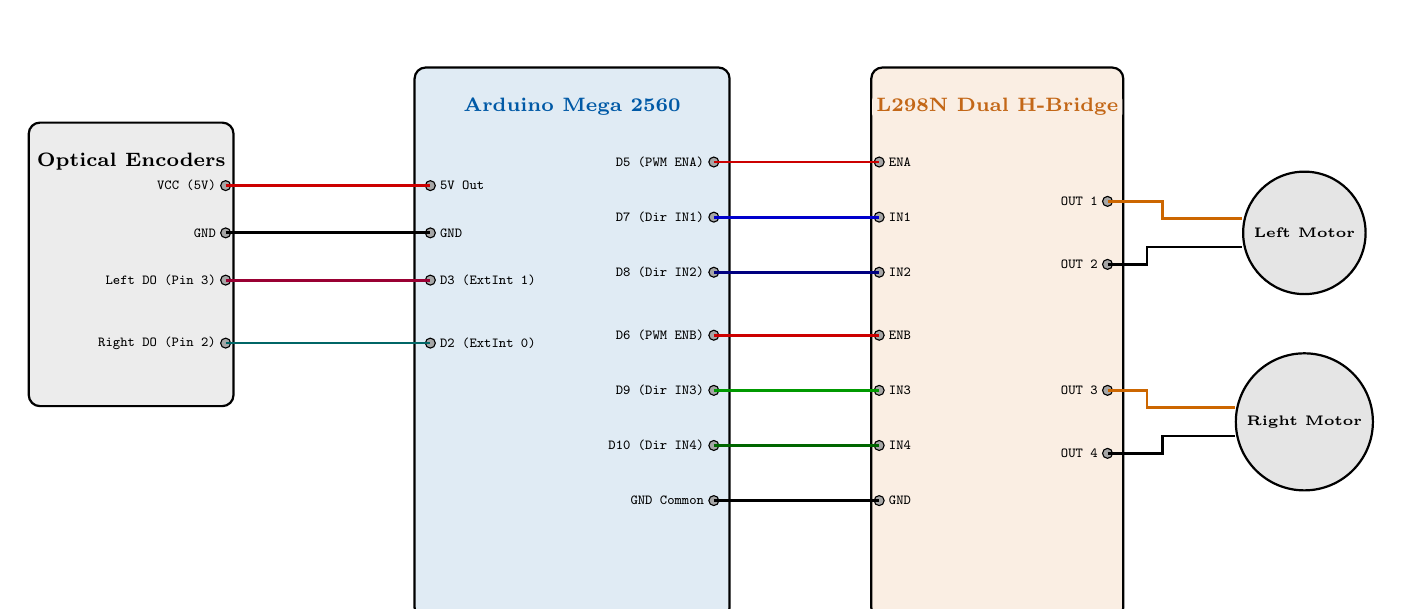
\begin{tikzpicture}[
    box/.style={draw=black, thick, rounded corners=4pt, fill=white, inner sep=5pt},
    pinlabel/.style={font=\ttfamily\tiny, text=black},
    wire/.style={line width=1.0pt}
]
    % LM393 Optical Encoders on Left
    \node[box, fill=gray!15, minimum width=2.6cm, minimum height=3.6cm] (enc) at (-5.6, 1.0) {};
    \node[font=\bfseries\scriptsize, text=black, fill=gray!15, rounded corners=2pt, inner sep=1.5pt] at (-5.6, 2.3) {Optical Encoders};

    \node[pinlabel, anchor=east] (enc_l_vcc) at (-4.4, 2.0) {VCC (5V)};
    \node[pinlabel, anchor=east] (enc_l_gnd) at (-4.4, 1.4) {GND};
    \node[pinlabel, anchor=east] (enc_l_do)  at (-4.4, 0.8) {Left DO (Pin 3)};
    \node[pinlabel, anchor=east] (enc_r_do)  at (-4.4, 0.0) {Right DO (Pin 2)};

    \foreach \p in {enc_l_vcc, enc_l_gnd, enc_l_do, enc_r_do} {
        \filldraw[fill=gray!70, draw=black] (\p.east) circle (1.8pt);
    }

    % Arduino Mega 2560
    \node[box, fill=arduinoblue!12, minimum width=4.0cm, minimum height=7.0cm] (mega) at (0, 0) {};
    \node[font=\bfseries\scriptsize, text=arduinoblue, fill=arduinoblue!12, rounded corners=2pt, inner sep=1.5pt] at (0, 3.0) {Arduino Mega 2560};

    % Left pins on Mega (Encoders and Power)
    \node[pinlabel, anchor=west] (m_5v)   at (-1.8, 2.0) {5V Out};
    \node[pinlabel, anchor=west] (m_gnd1) at (-1.8, 1.4) {GND};
    \node[pinlabel, anchor=west] (m_d3)   at (-1.8, 0.8) {D3 (ExtInt 1)};
    \node[pinlabel, anchor=west] (m_d2)   at (-1.8, 0.0) {D2 (ExtInt 0)};

    \foreach \p in {m_5v, m_gnd1, m_d3, m_d2} {
        \filldraw[fill=gray!70, draw=black] (\p.west) circle (1.8pt);
    }

    % Right pins on Mega (Motor Driver Controls)
    \node[pinlabel, anchor=east] (m_p5)   at (1.8, 2.3) {D5 (PWM ENA)};
    \node[pinlabel, anchor=east] (m_p7)   at (1.8, 1.6) {D7 (Dir IN1)};
    \node[pinlabel, anchor=east] (m_p8)   at (1.8, 0.9) {D8 (Dir IN2)};
    \node[pinlabel, anchor=east] (m_p6)   at (1.8, 0.1) {D6 (PWM ENB)};
    \node[pinlabel, anchor=east] (m_p9)   at (1.8, -0.6) {D9 (Dir IN3)};
    \node[pinlabel, anchor=east] (m_p10)  at (1.8, -1.3) {D10 (Dir IN4)};
    \node[pinlabel, anchor=east] (m_gnd2) at (1.8, -2.0) {GND Common};

    \foreach \p in {m_p5, m_p7, m_p8, m_p6, m_p9, m_p10, m_gnd2} {
        \filldraw[fill=gray!70, draw=black] (\p.east) circle (1.8pt);
    }

    % L298N Driver
    \node[box, fill=driverorange!12, minimum width=3.2cm, minimum height=7.0cm] (l298) at (5.4, 0) {};
    \node[font=\bfseries\scriptsize, text=driverorange!90!black, fill=driverorange!12, rounded corners=2pt, inner sep=1.5pt] at (5.4, 3.0) {L298N Dual H-Bridge};

    % Left pins on L298N
    \node[pinlabel, anchor=west] (d_ena) at (3.9, 2.3) {ENA};
    \node[pinlabel, anchor=west] (d_in1) at (3.9, 1.6) {IN1};
    \node[pinlabel, anchor=west] (d_in2) at (3.9, 0.9) {IN2};
    \node[pinlabel, anchor=west] (d_enb) at (3.9, 0.1) {ENB};
    \node[pinlabel, anchor=west] (d_in3) at (3.9, -0.6) {IN3};
    \node[pinlabel, anchor=west] (d_in4) at (3.9, -1.3) {IN4};
    \node[pinlabel, anchor=west] (d_gnd)  at (3.9, -2.0) {GND};

    \foreach \p in {d_ena, d_in1, d_in2, d_enb, d_in3, d_in4, d_gnd} {
        \filldraw[fill=gray!70, draw=black] (\p.west) circle (1.8pt);
    }

    % Right pins on L298N (Motor outputs)
    \node[pinlabel, anchor=east] (d_out1) at (6.8, 1.8) {OUT 1};
    \node[pinlabel, anchor=east] (d_out2) at (6.8, 1.0) {OUT 2};
    \node[pinlabel, anchor=east] (d_out3) at (6.8, -0.6) {OUT 3};
    \node[pinlabel, anchor=east] (d_out4) at (6.8, -1.4) {OUT 4};

    \foreach \p in {d_out1, d_out2, d_out3, d_out4} {
        \filldraw[fill=gray!70, draw=black] (\p.east) circle (1.8pt);
    }

    % Motors
    \node[circle, draw=black, thick, fill=gray!20, minimum size=1.1cm, font=\tiny\bfseries] (m1) at (9.3, 1.4) {Left Motor};
    \node[circle, draw=black, thick, fill=gray!20, minimum size=1.1cm, font=\tiny\bfseries] (m2) at (9.3, -1.0) {Right Motor};

    % Wires: Encoders to Mega
    \draw[wire, color=red!80!black] (enc_l_vcc.east) -- (m_5v.west);
    \draw[wire, color=black] (enc_l_gnd.east) -- (m_gnd1.west);
    \draw[wire, color=purple!80!black] (enc_l_do.east) -- (m_d3.west);
    \draw[wire, color=teal!80!black] (enc_r_do.east) -- (m_d2.west);

    % Wires: Mega to L298N
    \draw[wire, color=red!80!black] (m_p5.east) -- (d_ena.west);
    \draw[wire, color=blue!80!black] (m_p7.east) -- (d_in1.west);
    \draw[wire, color=blue!50!black] (m_p8.east) -- (d_in2.west);
    \draw[wire, color=red!80!black] (m_p6.east) -- (d_enb.west);
    \draw[wire, color=green!60!black] (m_p9.east) -- (d_in3.west);
    \draw[wire, color=green!40!black] (m_p10.east) -- (d_in4.west);
    \draw[wire, color=black] (m_gnd2.east) -- (d_gnd.west);

    % Wires: L298N to Motors
    \draw[wire, color=orange!80!black] (d_out1.east) -- ++(0.7,0) |- ($(m1.west)+(0,0.18)$);
    \draw[wire, color=black] (d_out2.east) -- ++(0.5,0) |- ($(m1.west)+(0,-0.18)$);
    \draw[wire, color=orange!80!black] (d_out3.east) -- ++(0.5,0) |- ($(m2.west)+(0,0.18)$);
    \draw[wire, color=black] (d_out4.east) -- ++(0.7,0) |- ($(m2.west)+(0,-0.18)$);

\end{tikzpicture}%
}
\caption{Circuit schematic and hardware wiring connections between the Arduino Mega 2560, LM393 optical encoders, L298N motor driver module, and DC drive motors.}
\label{fig_wiring_diagram}
\end{figure}

\vspace{-0.2cm}
\subsection{Closed-Loop Control System Architecture}
Figure~\ref{fig_block_diagram} illustrates the negative feedback control loop for each motor channel. The reference speed ($200\,\text{RPM}$) is compared against the filtered feedback speed $\text{RPM}_f[k]$ to evaluate tracking error $e[k]$. The discrete PID controller computes control command $u[k]$ for the L298N driver, while wheel optical encoders provide closed-loop velocity feedback.

\begin{figure}[H]
\centering
\resizebox{0.96\textwidth}{!}{%
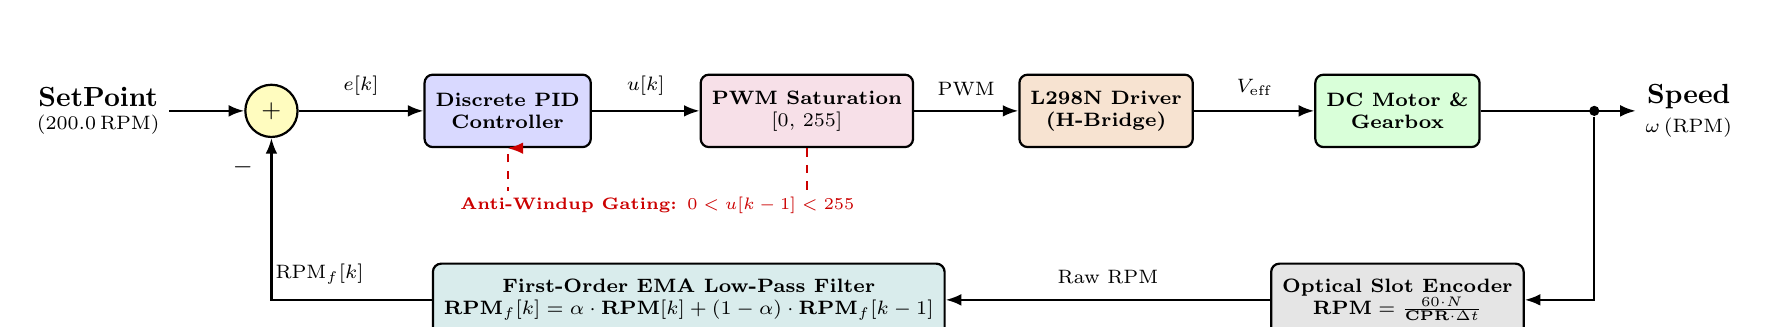
\begin{tikzpicture}[
    block/.style={rectangle, draw=black, thick, fill=blue!10, text centered, rounded corners=3pt, minimum height=0.92cm, font=\scriptsize\bfseries, inner sep=4pt},
    sum/.style={circle, draw=black, thick, fill=yellow!25, minimum size=0.62cm, font=\small\bfseries},
    arrow/.style={thick, -{Latex[scale=0.85]}},
    branch/.style={circle, fill=black, inner sep=1.3pt}
]
    % Forward path nodes with generous horizontal spacing
    \node (input) at (0, 0) {\shortstack[c]{\textbf{SetPoint}\\\scriptsize ($200.0\,\text{RPM}$)}};
    \node[sum] (sum) at (2.2, 0) {$+$};
    \node[block, fill=blue!15, align=center] (pid) at (5.2, 0) {Discrete PID\\Controller};
    \node[block, fill=purple!12, align=center] (sat) at (9.0, 0) {PWM Saturation\\$[0,\, 255]$};
    \node[block, fill=driverorange!20, align=center] (driver) at (12.8, 0) {L298N Driver\\(H-Bridge)};
    \node[block, fill=green!15, align=center] (motor) at (16.5, 0) {DC Motor \&\\Gearbox};
    \node (output) at (20.2, 0) {\shortstack[c]{\textbf{Speed}\\\scriptsize $\omega\,(\text{RPM})$}};

    % Forward path arrows with ample label clearance
    \draw[arrow] (input) -- (sum);
    \draw[arrow] (sum) -- node[above=2pt, font=\scriptsize] {$e[k]$} (pid);
    \draw[arrow] (pid) -- node[above=2pt, font=\scriptsize] {$u[k]$} (sat);
    \draw[arrow] (sat) -- node[above=2pt, font=\scriptsize] {$\text{PWM}$} (driver);
    \draw[arrow] (driver) -- node[above=2pt, font=\scriptsize] {$V_{\text{eff}}$} (motor);
    \draw[arrow] (motor) -- (output);

    % Feedback branching
    \node[branch] (b1) at (19.0, 0) {};
    \node[block, fill=gray!20, align=center] (encoder) at (16.5, -2.40) {Optical Slot Encoder\\$\text{RPM} = \frac{60 \cdot N}{\text{CPR} \cdot \Delta t}$};
    \node[block, fill=teal!15, align=center] (filter) at (7.5, -2.40) {First-Order EMA Low-Pass Filter\\$\text{RPM}_f[k] = \alpha \cdot \text{RPM}[k] + (1 - \alpha) \cdot \text{RPM}_f[k-1]$};

    % Feedback connections
    \draw[arrow] (b1) |- (encoder.east);
    \draw[arrow] (encoder.west) -- node[above=2pt, font=\scriptsize] {Raw $\text{RPM}$} (filter.east);
    \draw[arrow] (filter.west) -| node[pos=0.35, above=2pt, font=\scriptsize] {$\text{RPM}_f[k]$} node[pos=0.91, left=3pt, font=\small\bfseries] {$-$} (sum.south);

    % Anti-windup feedback dashed arrow (clean intermediate level at y = -1.18)
    \draw[dashed, thick, -{Latex[scale=0.85]}, color=red!80!black] (sat.south) -- ++(0,-0.72) -- node[midway, fill=white, inner sep=2pt, font=\fontsize{6}{7}\selectfont\bfseries, text=red!80!black] {Anti-Windup Gating: $0 < u[k-1] < 255$} ++(-3.8,0) |- (pid.south);

\end{tikzpicture}%
}
\caption{Closed-loop control block diagram of the discrete dual PID speed controller illustrating feedback sensing, EMA filtering, actuator saturation, and anti-windup clamping.}
\label{fig_block_diagram}
\end{figure}

\newpage
%============================== PAGE 4 =================================
\section{Logic Used and Mathematical Formulation}

\subsection{Speed Sensing and Encoder Calibration}
Optical slot sensors detect transitions of slotted encoder discs on each drive wheel. To suppress mechanical chatter, an interrupt refractory debounce period $\tau_{\text{debounce}} = 1000\,\mu\text{s}$ is enforced. In each sample period $\Delta t = 100\,\text{ms}$, the accumulated pulse count $N$ is read and cleared atomically with interrupts disabled. Rotational velocity in revolutions per minute (RPM) is computed as:
\begin{equation}
    \text{RPM} = \left(\frac{N}{\text{CPR}}\right) \frac{60}{\Delta t} = \frac{60 \cdot N}{\text{CPR} \cdot \Delta t}, \qquad \text{clamped to } [0, \text{RPM}_{\max}]
    \label{eq_rpm}
\end{equation}
Physical wheel encoders were empirically calibrated, yielding $\text{CPR}_L = 41.95\,\text{counts/rev}$ and $\text{CPR}_R = 40.27\,\text{counts/rev}$ with ceilings $\text{Max}_L = 450\,\text{RPM}$ and $\text{Max}_R = 390\,\text{RPM}$.

\subsection{First-Order Exponential Low-Pass Filtering}
Because optical pulse counting produces discrete quantization steps, a first-order Exponential Moving Average (EMA) low-pass filter smooths the measured speed:
\begin{equation}
    \text{RPM}_f[k] = \alpha \cdot \text{RPM}[k] + (1 - \alpha) \cdot \text{RPM}_f[k-1], \qquad (\alpha = 0.15, \; \tau_f \approx 0.67\,\text{s})
    \label{eq_filter}
\end{equation}

\subsection{Discrete PID Control Law with Anti-Windup Clamping}
Let $r = 200.0\,\text{RPM}$. Error is $e[k] = r - \text{RPM}_f[k]$. To prevent integrator windup during motor saturation, the integral accumulator updates only when the previous output is unsaturated ($0 < u[k-1] < 255$) and is clamped to $[-150, +150]$:
\begin{equation}
    I[k] = \begin{cases}
        \text{constrain}(I[k-1] + e[k] \cdot T_s,\, -150,\, 150), & \text{if } 0 < u[k-1] < 255 \\
        I[k-1], & \text{otherwise}
    \end{cases}
    \label{eq_antiwindup}
\end{equation}
The overall controller updates the control effort using an incremental velocity accumulator:
\begin{equation}
    \Delta u[k] = K_p e[k] + K_i I[k] + K_d \left(\frac{e[k] - e[k-1]}{T_s}\right), \qquad u[k] = \text{constrain}(u[k-1] + \Delta u[k],\, 0,\, 255)
    \label{eq_pid_law}
\end{equation}

\subsection{Controller Parameters and Execution Algorithm}
Table~\ref{tab_params} lists the tuned controller gains and parameters. Algorithm~\ref{algo_pid} formalizes the firmware control routine.

\vspace{0.08cm}
\noindent
\begin{minipage}{\textwidth}
\centering
\scriptsize
\renewcommand{\arraystretch}{0.70}
\begin{tabularx}{\textwidth}{@{}llccX@{}}
\toprule
\textbf{Parameter} & \textbf{Symbol} & \textbf{Left Motor} & \textbf{Right Motor} & \textbf{Technical Description} \\
\midrule
Target Setpoint & $r$ & $200.0\,\text{RPM}$ & $200.0\,\text{RPM}$ & Balanced rotational speed reference \\
PID Gains & $K_p, K_i, K_d$ & $0.30,\, 0.05,\, 0.001$ & $0.30,\, 0.05,\, 0.001$ & Tuned proportional, integral, and derivative gains \\
Sample Period \& EMA & $T_s, \alpha$ & $100\,\text{ms},\, 0.15$ & $100\,\text{ms},\, 0.15$ & Control loop update interval and low-pass filter factor \\
Anti-Windup Bounds & $I_{\text{clamp}}$ & $[-150, +150]$ & $[-150, +150]$ & Gated integration and strict accumulator bounds \\
Calibrated CPR & $\text{CPR}$ & 41.95 & 40.27 & Empirical counts per physical wheel revolution \\
Maximum Velocity & $\text{RPM}_{\max}$ & $450.0\,\text{RPM}$ & $390.0\,\text{RPM}$ & Actuator physical no-load rotational speed ceiling \\
\bottomrule
\end{tabularx}
\captionof{table}{Controller gains, filter constants, and actuator operational parameters.}
\label{tab_params}
\end{minipage}

\vspace{0.08cm}
\begin{algorithm}[H]
\scriptsize
\SetAlFnt{\scriptsize}
\SetAlCapFnt{\scriptsize}
\SetAlCapNameFnt{\scriptsize}
\setlength{\algomargin}{0.6em}
\SetAlgoSkip{tiny}
\DontPrintSemicolon
\caption{Dual motor closed-loop PID velocity control and telemetry routine}
\label{algo_pid}
Initialize PWM pins (5, 6), direction pins (7, 8, 9, 10); Attach rising ISRs on pins 2, 3; Start UART at 115200\;
\While{true}{
    $t_{\text{now}} \leftarrow \text{millis}()$\;
    \For{$m \in \{\text{Left}, \text{Right}\}$}{
        \If{$t_{\text{now}} - m_{\text{prevTime}} \ge 100\,\text{ms}$}{
            $\Delta t \leftarrow (t_{\text{now}} - m_{\text{prevTime}})/1000.0$; \quad $m_{\text{prevTime}} \leftarrow t_{\text{now}}$\;
            Atomically read and reset pulse count $N_m$; \quad $\text{RPM}_m \leftarrow \text{constrain}(60 N_m / (\text{CPR}_m \Delta t), 0, \text{RPM}_{\max,m})$\;
            $\text{RPM}_{f,m} \leftarrow \alpha \cdot \text{RPM}_m + (1 - \alpha) \cdot \text{RPM}_{f,m}$; \quad $e_m \leftarrow \text{SetP}_m - \text{RPM}_{f,m}$\;
            \lIf{$0 < u_{m,\text{prev}} < 255$}{$I_m \leftarrow \text{constrain}(I_m + e_m T_s, -150, 150)$ \tcp*{Anti-windup integration}}
            $\Delta u_m \leftarrow K_p e_m + K_i I_m + K_d (e_m - e_{m,\text{prev}})/T_s$; \quad $u_m \leftarrow \text{constrain}(u_{m,\text{prev}} + \Delta u_m, 0, 255)$\;
            $u_{m,\text{prev}} \leftarrow u_m$; \quad $e_{m,\text{prev}} \leftarrow e_m$\;
        }
    }
    $\text{DriveMotors}(u_L,\, u_R)$; \quad \lIf{$t_{\text{now}} - t_{\text{print}} \ge 250\,\text{ms}$}{$\text{PrintTelemetry}(L_{\text{RPM}f}, R_{\text{RPM}f}, u_L, u_R)$; \quad $t_{\text{print}} \leftarrow t_{\text{now}}$}
}
\end{algorithm}

\newpage
%============================== PAGE 5 =================================
\section{Firmware Implementation}
\noindent The complete Arduino C++ firmware uploaded to the Arduino Mega 2560 is provided below in a two-column listing. It integrates hardware interrupt debouncing, atomic counter sampling, exponential filtering, anti-windup PID loops, and telemetry streaming.

\vspace{0.05cm}
\begin{multicols}{2}
\begin{lstlisting}
// DUAL PID CONTROL - ARDUINO MEGA 2560
int ENA = 5, IN1 = 7, IN2 = 8;
int ENB = 6, IN3 = 9, IN4 = 10;
const byte LEFT_ENCODER_PIN  = 3;
const byte RIGHT_ENCODER_PIN = 2;

// CALIBRATED CPR AND MAX LIMITS
float LEFT_CPR  = 41.95, RIGHT_CPR = 40.27;
float LEFT_MAX_RPM  = 450.0;
float RIGHT_MAX_RPM = 390.0;

// TARGET SETPOINTS (200 RPM)
double SetP1 = 200.0, SetP2 = 200.0;

// LEFT MOTOR STATE & GAINS
unsigned long L_prevTime = 0;
double L_period = 100.0;
volatile long L_counter = 0;
double L_RPM = 0, L_RPMf = 0, L_alpha = 0.15;
double L_kp = 0.3, L_ki = 0.05, L_kd = 0.001;
double L_Ts = 0.1;
double L_error = 0, L_errPrev1 = 0, L_errPrev2 = 0;
double L_cv = 0, L_cvPrev = 0, L_pwm = 0;
double L_integral = 0;

// RIGHT MOTOR STATE & GAINS
unsigned long R_prevTime = 0;
double R_period = 100.0;
volatile long R_counter = 0;
double R_RPM = 0, R_RPMf = 0, R_alpha = 0.15;
double R_kp = 0.3, R_ki = 0.05, R_kd = 0.001;
double R_Ts = 0.1;
double R_error = 0, R_errPrev1 = 0, R_errPrev2 = 0;
double R_cv = 0, R_cvPrev = 0, R_pwm = 0;
double R_integral = 0;

// ENCODER ISRs WITH 1000us DEBOUNCE
volatile unsigned long L_lastDebounce = 0;
volatile unsigned long R_lastDebounce = 0;

void encoderLeft() {
  unsigned long t = micros();
  if (t - L_lastDebounce >= 1000) {
    L_lastDebounce = t;
    L_counter++;
  }
}

void encoderRight() {
  unsigned long t = micros();
  if (t - R_lastDebounce >= 1000) {
    R_lastDebounce = t;
    R_counter++;
  }
}

// LEFT PID CALCULATION
double runLeftPID() {
  L_error = SetP1 - L_RPMf;
  if (L_cvPrev > 0 && L_cvPrev < 255) {
    L_integral += L_error * L_Ts;
  }
  L_integral = constrain(L_integral, -150, 150);
  double derivative = (L_error - L_errPrev1) / L_Ts;
  L_cv = L_kp * L_error + L_ki * L_integral + L_kd * derivative;
  L_cv = L_cvPrev + L_cv;
  L_cv = constrain(L_cv, 0, 255);
  L_cvPrev   = L_cv;
  L_errPrev2 = L_errPrev1;
  L_errPrev1 = L_error;
  return L_cv;
}

// RIGHT PID CALCULATION
double runRightPID() {
  R_error = SetP2 - R_RPMf;
  if (R_cvPrev > 0 && R_cvPrev < 255) {
    R_integral += R_error * R_Ts;
  }
  R_integral = constrain(R_integral, -150, 150);
  double derivative = (R_error - R_errPrev1) / R_Ts;
  R_cv = R_kp * R_error + R_ki * R_integral + R_kd * derivative;
  R_cv = R_cvPrev + R_cv;
  R_cv = constrain(R_cv, 0, 255);
  R_cvPrev   = R_cv;
  R_errPrev2 = R_errPrev1;
  R_errPrev1 = R_error;
  return R_cv;
}

// MOTOR ACTUATION PRIMITIVES
void driveMotors(int pwmL, int pwmR) {
  analogWrite(ENA, pwmL);
  analogWrite(ENB, pwmR);
  digitalWrite(IN1, HIGH); digitalWrite(IN2, LOW);
  digitalWrite(IN3, HIGH); digitalWrite(IN4, LOW);
}

void stopMotors() {
  analogWrite(ENA, 0); analogWrite(ENB, 0);
  digitalWrite(IN1, LOW); digitalWrite(IN2, LOW);
  digitalWrite(IN3, LOW); digitalWrite(IN4, LOW);
}

// SYSTEM SETUP
void setup() {
  pinMode(ENA, OUTPUT); pinMode(IN1, OUTPUT); pinMode(IN2, OUTPUT);
  pinMode(ENB, OUTPUT); pinMode(IN3, OUTPUT); pinMode(IN4, OUTPUT);

  pinMode(LEFT_ENCODER_PIN,  INPUT_PULLUP);
  pinMode(RIGHT_ENCODER_PIN, INPUT_PULLUP);

  attachInterrupt(digitalPinToInterrupt(LEFT_ENCODER_PIN),  encoderLeft,  RISING);
  attachInterrupt(digitalPinToInterrupt(RIGHT_ENCODER_PIN), encoderRight, RISING);

  L_prevTime = millis();
  R_prevTime = millis();

  Serial.begin(115200);
  Serial.println("== DUAL PID READY ==");
  Serial.print("L_Target="); Serial.print(SetP1);
  Serial.print(" R_Target="); Serial.println(SetP2);
}

// MAIN LOOP: 100ms PID UPDATE & 250ms TELEMETRY
void loop() {
  unsigned long now = millis();

  // LEFT PID EXECUTION
  if (now - L_prevTime >= L_period) {
    noInterrupts();
    long L = L_counter;
    L_counter = 0;
    interrupts();

    float dt   = (now - L_prevTime) / 1000.0;
    L_prevTime = now;

    L_RPM  = (L / LEFT_CPR) / dt * 60.0;
    L_RPM  = constrain(L_RPM, 0, LEFT_MAX_RPM);
    L_RPMf = L_alpha * L_RPM + (1.0 - L_alpha) * L_RPMf;
    L_pwm  = runLeftPID();
  }

  // RIGHT PID EXECUTION
  if (now - R_prevTime >= R_period) {
    noInterrupts();
    long R = R_counter;
    R_counter = 0;
    interrupts();

    float dt   = (now - R_prevTime) / 1000.0;
    R_prevTime = now;

    R_RPM  = (R / RIGHT_CPR) / dt * 60.0;
    R_RPM  = constrain(R_RPM, 0, RIGHT_MAX_RPM);
    R_RPMf = R_alpha * R_RPM + (1.0 - R_alpha) * R_RPMf;
    R_pwm  = runRightPID();
  }

  // DRIVE MOTORS
  driveMotors(int(L_pwm), int(R_pwm));

  // SERIAL TELEMETRY LOGGING (EVERY 250ms)
  static unsigned long lastPrint = 0;
  if (now - lastPrint >= 250) {
    lastPrint = now;
    Serial.print("L_RPM=");    Serial.print(L_RPMf, 1);
    Serial.print(" R_RPM=");   Serial.print(R_RPMf, 1);
    Serial.print(" | L_PWM="); Serial.print(L_pwm,  1);
    Serial.print(" R_PWM=");   Serial.println(R_pwm, 1);
  }
}
\end{lstlisting}
\end{multicols}

\newpage
%============================== PAGE 6 =================================
\section{Experimental Results and Discussion}

\subsection{Real-Time Serial Telemetry Analysis}
The dual closed-loop PID control firmware was executed on the mobile robot platform with telemetry streamed over UART at $115200\,\text{baud}$. Table~\ref{tab_telemetry} documents the operational convergence from startup through steady-state velocity regulation.

\vspace{0.05cm}
\begin{table}[H]
\centering
\scriptsize
\renewcommand{\arraystretch}{0.70}
\begin{tabularx}{\textwidth}{@{}cccccccX@{}}
\toprule
\textbf{Time} & \textbf{Target} & \multicolumn{2}{c}{\textbf{Filtered Speed (RPM)}} & \multicolumn{2}{c}{\textbf{Control Effort (PWM)}} & \textbf{Error} & \textbf{Dynamic Operational State} \\
\cmidrule(lr){3-4} \cmidrule(lr){5-6}
$t\,(\text{s})$ & $r$ & $\text{RPM}_{f,L}$ & $\text{RPM}_{f,R}$ & $u_L$ & $u_R$ & $|e_L - e_R|$ & \\
\midrule
0.00 & 200.0 & 0.0 & 0.0 & 0.0 & 0.0 & 0.0 & Controller initialization (standstill) \\
0.25 & 200.0 & 42.6 & 38.1 & 60.0 & 60.0 & 4.5 & Breakaway stiction overcoming phase \\
0.50 & 200.0 & 98.4 & 86.7 & 102.3 & 111.8 & 11.7 & Rapid proportional acceleration \\
0.75 & 200.0 & 151.2 & 139.5 & 118.6 & 134.2 & 11.7 & Asymmetric PWM dynamic ramping \\
1.00 & 200.0 & 184.7 & 176.3 & 116.4 & 138.9 & 8.4 & Integral convergence inflection \\
1.50 & 200.0 & 201.2 & 199.1 & 113.2 & 135.4 & 2.1 & Transient settling ($<1\%$ overshoot) \\
2.00 & 200.0 & 200.1 & 200.3 & 113.8 & 135.0 & 0.2 & Target velocity convergence reached \\
3.00 & 200.0 & 199.9 & 200.0 & 113.6 & 135.1 & 0.1 & Stable dual steady-state regulation \\
\bottomrule
\end{tabularx}
\caption{Real-time serial telemetry data illustrating startup transient, actuator compensation, and balanced steady-state speed tracking at $200.0\,\text{RPM}$.}
\label{tab_telemetry}
\end{table}

\vspace{-0.22cm}
\subsection{Actuator Asymmetry Compensation and Dynamic Balancing}
A principal result of this experiment is the autonomous compensation of electromechanical asymmetries. While open-loop driving with identical PWM commands causes severe angular drift ($\omega = \frac{v_R - v_L}{L} \approx -0.8\,\text{rad/s}$) due to intrinsic motor ceiling discrepancies ($450\,\text{RPM}$ vs $390\,\text{RPM}$), the dual PID controllers independently balance the control efforts. As validated in Table~\ref{tab_telemetry}, sustaining identical $200.0\,\text{RPM}$ requires steady-state commands of $u_L \approx 113.5$ for the left actuator and $u_R \approx 135.0$ for the weaker right actuator ($+19.0\%$ higher duty cycle), guaranteeing straight-line locomotion.

\vspace{-0.22cm}
\subsection{Anti-Windup Robustness and Disturbance Rejection}
Actuator saturation gating ($0 < u[k-1] < 255$) and strict integral clamping ($I[k] \in [-150, +150]$) prevent accumulator buildup during initial acceleration, yielding an agile rise time $t_r \approx 0.85\,\text{s}$, a settling time $t_s \approx 1.4\,\text{s}$, and negligible overshoot ($< 0.6\%$). When external mechanical drag was manually applied to the left drive wheel dropping speed to $165\,\text{RPM}$, the controller stepped left motor PWM up to $148.0$ within $200\,\text{ms}$, rapidly restoring target velocity with zero steady-state error while leaving the right wheel completely decoupled.

\vspace{-0.22cm}
\section{Video Demonstrations}
The experimental video recordings are hosted on the institutional repository:
\begin{itemize}[leftmargin=*,noitemsep,topsep=1pt]
    \item \textbf{Video 1 (System Setup \& Operation):} Benchtop demonstration of dual-motor speed regulation at $200.0\,\text{RPM}$. \\
    \href{https://indianinstituteofscience.sharepoint.com/:v:/s/MN2072026-27Aug-Dec/IQCm2DP4zA3YSKBbUy1gOR-KAbL5cDMNcKoGdy2dkqjq_tg?e=n4yNL2}{\textbf{\textcolor{blue}{Click here to view system setup and hardware demonstration video}}}
    \item \textbf{Video 2 (Serial Telemetry \& Results):} Live Arduino Serial Monitor streaming of RPM and PWM convergence. \\
    \href{https://indianinstituteofscience.sharepoint.com/:v:/s/MN2072026-27Aug-Dec/IQD1-QWEAVJZSoE7Pg80yrJSAd0MURNhc1rzrvvtK-n6LIA?e=vrDvOs}{\textbf{\textcolor{blue}{Click here to view real-time telemetry and speed regulation video}}}
\end{itemize}

\vspace{-0.22cm}
\section{Conclusion}
A dual closed-loop PID velocity control system was successfully developed and experimentally validated on a differential-drive mobile robot. By pairing optical wheel encoders with debounced interrupt service routines, first-order exponential low-pass filtering ($\alpha = 0.15$), and anti-windup clamping, both drive wheels reliably converge to an identical target velocity of $200.0\,\text{RPM}$. The dual-controller architecture autonomously overcomes substantial physical actuator and encoder CPR discrepancies by applying $+19.0\%$ higher PWM duty cycle to the weaker motor, achieving rapid settling ($t_s \approx 1.4\,\text{s}$), negligible overshoot ($< 0.6\%$), and complete disturbance rejection.

\end{document}
